%% LyX 1.5.6 created this file.  For more info, see http://www.lyx.org/.
%% Do not edit unless you really know what you are doing.
\documentclass[a4paper,twoside,twocolumn,brazil,portuges,a4paper]{article}
\usepackage[T1]{fontenc}
\usepackage[utf8]{inputenc}
\usepackage{textcomp}
\usepackage{url}
\usepackage{color}
\usepackage{graphicx}
\usepackage[numbers]{natbib}

\makeatletter

%%%%%%%%%%%%%%%%%%%%%%%%%%%%%% LyX specific LaTeX commands.
%% Because html converters don't know tabularnewline
\providecommand{\tabularnewline}{\\}

%%%%%%%%%%%%%%%%%%%%%%%%%%%%%% User specified LaTeX commands.
% http://swasr.googlecode.com/svn/trunk/latex/artigo1/artigo1.pdf
%\documentclass{acm_proc_article-sp}



%\usepackage[portuguese]{babel}


\usepackage{url}


\hyphenation{pa-ra-me-tri-zá-veis ba-se-a-da ve-ros-si-mi-lhan-ça o-ri-en-ta-das não-o-ri-en-ta-das subs-ti-tu-í-dos a-de-qua-da-men-te mo-de-los}

%the story is not what you did, but rather
%  what you show, new ideas, new insights
%  why interesting, important?
%why is the story of interest to others?
%  universal truths, hot topic, surprises or unexpected results?

% == PLANEJAMENTO DO EXPERIMENTO ==
% 
% INGREDIENTES
%
%   Dois sistemas, um pequeno (?) e um maior (IRPF)
%   Modelos de geração de redes com estrutura de módulos embutida: Rodrigo2008 e Lancichinetti
%   Modelos sem estrutura de módulos: barabasi, bollobas, configuration model.
%
% MODO DE PREPARO
%
%   Analisar métricas dos sistemas (distribuição de graus, distribuição do coeficiente de clustering, correlação de graus).
%   Extrair a arquitetura dos sistemas: quais são os módulos e quais módulos se relacionam. Analisar a distribuição dos tamanhos dos módulos.
%   "Tunar" os parâmetros dos modelos para gerar redes com as mesmas métricas dos sistemas reais
%   Rodar os modelos diversas vezes com os parâmetros encontrados para gerar diversas redes para cada sistema.
%   Comparar redes sintéticas com as redes reais correspondentes através da distância entre redes de Garcia.
% 
% RESULTADOS
%
%   Modelos com estrutura de módulos embutida resultam em redes mais parecidas com as redes reais do que os modelos sem módulos? (Em outras palavras: a informação sobre tamanhos dos módulos e a maneira como os módulos se ligam realmente são uma vantagem?)
%   As redes sintéticas são realistas? Quais as diferenças entre as sintéticas e as reais?
%   Os módulos das redes sintéticas também podem ser decompostos em módulos, como nas redes reais?
%
% O QUE MAIS
%
%   Ver no wiki as observações subjetivas sobre os modelos.
%   Começar pelo sistema pequeno, pra obter resultados mais rápidos, e então reproduzir o método com o sistema grande
%   A implementação do modelo de Rodrigo2008 precisa ser revista pra ficar mais eficiente (está muito lento!)
%   Podemos usar uma distância de Garcia usando o coeficiente de clustering em vez de usar a distância propriamente dita.

\makeatother

\usepackage{babel}

\begin{document}

\title{Modelos Estocásticos para Síntese de Sistemas de Software Organizados
em Módulos \\
 {*}DRAFT v3{*}}


\author{Rodrigo Rocha Gomes e Souza}

\maketitle
\begin{abstract}
Algoritmos de modularização de \emph{software} procuram identificar
a estrutura de módulos de um sistema de \emph{software} a partir de
sua implementação. Infelizmente, dada a dificuldade de se encontrar
sistemas cuja organização modular é bem documentada, há poucos estudos
dedicados a testar empiricamente esses algoritmos. Propomos suprir
essa escassez através do uso de modelos estocásticos capazes de gerar
sistemas de \emph{software} organizados em módulos para servirem como
conjunto de teste. Neste artigo apresentamos dois modelos que cumprem
essa função --- um deles inédito --- e concluímos através de um experimento
que um dos modelos produz sistemas semelhantes a sistemas reais, ao
menos do ponto de vista dos algoritmos de modularização.
\end{abstract}

\section{Introdução}

A divisão conceitual de um sistema de \emph{software} em módulos é
uma informação valiosa durante o seu desenvolvimento, sobretudo para
a divisão de tarefas entre desenvolvedores \citep{Clements2002}.
Essa informação muitas vezes não é documentada adequadamente e, à
medida que os desenvolvedores são substituídos, pode se perder. Por
essa razão foram propostos diversos algoritmos de modularização de
\emph{software}, os quais procuram identificar a organização em módulos
de um sistema de \emph{software} a partir de sua implementação \citep{Mancoridis1998,Andritsos2003,Maqbool2007}.

Espera-se que os algoritmos encontrem organizações modulares semelhantes
àquelas que seriam encontradas por especialistas nos sistemas analisados.
Uma forma de testar os algoritmos consiste, pois, em aplicá-los ao
código-fonte de um sistema cuja organização em módulos esteja documentada
e então comparar as duas estruturas de módulos \citet{Tzerpos1999}.
Infelizmente é difícil encontrar sistemas documentados nesse nível
de detalhe e por essa razão a avaliação empírica dos algoritmos de
modularização de \emph{software} ainda é incipiente. 

Para suprir a escassez de sistemas bem documentados, propomos o uso
de modelos estocásticos capazes de sintetizar sistemas de \emph{software}
organizados em módulos para servirem como conjunto de teste. Para
que essa abordagem seja bem-sucedida, no entanto, é preciso que os
sistemas sintéticos sejam realistas, isto é, semelhantes a sistemas
reais, ao menos do ponto de vista dos algoritmos de modularização.
Neste artigo apresentamos dois modelos --- um deles inédito --- e
avaliamos através de um experimento o realismo dos sistemas que eles
produzem.

A próxima seção apresenta o embasamento teórico deste trabalho. A
seguir, na seção \ref{sec:modelos}, descrevemos os modelos estocásticos
que sintetizam sistemas de \emph{software} organizados em módulos.
Na seção \ref{sec:experimento} relatamos o experimento realizado
para avaliar os modelos e os seus resultados. Por fim, discutimos
direções futuras para pesquisa.


\section{Teoria}

Sistemas de \emph{software}, no nível de implementação, são formados
por vários componentes que interagem entre si de diversas formas.
Sistemas implementados em linguagens orientadas a objetos, por exemplo,
são compostos por classes que interagem com outras classes através
de mecanismos como troca de mensagens e herança. As interações estabelecem
relações de dependência entre os componentes, de forma que cada componente
só funciona corretamente na presença dos componentes dos quais ele
depende. 

Para viabilizar o desenvolvimento de um sistema de \emph{software}
com muitos componentes é comum agrupá-los em módulos. Não existe um
critério unânime para realizar esse agrupamento, mas em geral se assume
que os módulos agrupam componentes que dependem mais uns dos outros
do que de componentes que pertencem a outros módulos. Esse padrão
de dependências permite que os módulos sejam desenvolvidos de forma
mais ou menos independente, possivelmente por equipes distintas.

A rede de dependências pode ser extraída automaticamente através de
ferramentas de análise estática de código-fonte ou código objeto.
A organização dos componentes em módulos, por outro lado, não é explicitamente
representada no código-fonte. O objetivo das ferramentas de modularização
de software é encontrar, a partir da rede de dependências de um sistema,
uma organização dos componentes em módulos que seja adequada para
apoiar o desenvolvimento do sistema. 

A rede de dependências entre componentes de um sistema de \emph{software}
pode ser representada por um grafo no qual os vértices representam
os componentes e as arestas representam as relações de dependência
entre os componentes. Neste trabalho usamos os termos rede e grafo
como sinônimos. A depender do nível de detalhe desejado, o grafo pode
ser não-orientado --- no qual considera-se que a relação de dependência
é simétrica --- ou orientado --- no qual as arestas possuem uma origem
e um destino bem definidos. Pode-se ainda associar a cada aresta um
número indicando o peso da dependência, o que caracteriza o grafo
como ponderado. A organização em módulos é representada através de
um particionamento do conjunto de vértices, no qual cada partição
representa um módulo. A Figura \ref{fig:rede} mostra um grafo orientado,
não-ponderado e organizado em módulos.

%
\begin{figure}
\noindent \begin{centering}
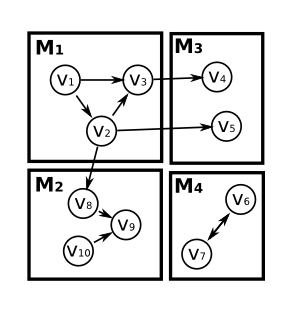
\includegraphics{rede}
\par\end{centering}

\caption{\selectlanguage{brazil}%
Representação gráfica de uma rede orientada organizada em quatro módulos.\selectlanguage{portuges}
}
\label{fig:rede}
\end{figure}


A arquitetura modular de um sistema organizado em módulos é um grafo
que representa os módulos e as dependências entre eles. Na arquitetura
modular há uma aresta de um módulo $M_{1}$ para um módulo $M_{2}$
somente se existe uma aresta de um vértice de $M_{1}$ para um vértice
de $M_{2}$. A Figura \ref{fig:arquitetura} mostra a arquitetura
modular da Figura \ref{fig:rede}.

%
\begin{figure}
\noindent \begin{centering}
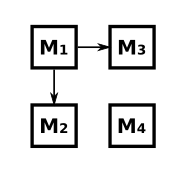
\includegraphics{arquitetura}
\par\end{centering}

\caption{\selectlanguage{brazil}%
A arquitetura modular da rede da Figura \ref{fig:rede}.\selectlanguage{portuges}
}
\label{fig:arquitetura}
\end{figure}


Pesquisas recentes mostram que redes de dependências entre componentes
possuem características comuns a redes complexas estudadas em diversos
domínios, tais como sociologia, biologia e linguística \citep{Myers2003,Valverde2003}.
Uma das características mais estudadas é a distribuição dos graus
dos vértices. Descobriu-se que, em diversas redes estudadas, essa
distribuição segue uma lei de potência, ou seja, o número de vértices
ligados a exatamente $k$ arestas é proporcional a $k^{-\gamma}$,
onde o expoente $\gamma$ varia tipicamente entre 2 e 3. Uma consequência
dessa distribuição é a presença de vértices cujo grau é muito superior
à média. 

As características comuns a redes de diversos domínios foram incorporadas
a vários modelos estocásticos de geração de redes \citep{Bollobas2003,Lancichinetti2008}.
As redes geradas por esses modelos podem ser interpretadas como redes
de dependências entre componentes.


\subsection{Distância entre Redes}

\textbf{\textcolor{red}{\large }}Embora métricas como o expoente
da distribuição de graus ($\gamma$) sejam úteis para caracterizar
redes, elas não são adequadas para se diferenciar duas redes. Não
é difícil encontrar redes que, embora possuam o mesmo número de vértices,
o mesmo número de arestas e o mesmo expoente $\gamma$, são muito
diferentes entre si. Por essa razão neste trabalho usamos uma métrica
de distância entre redes \citep{Andrade2008} para avaliar o quanto
uma rede sintética se parece com uma rede extraída de um sistema real.
Essa métrica se baseia no conceito de matrizes de vizinhança e se
aplica apenas a redes com o mesmo número de vértices.

Uma matriz de vizinhança de uma rede, $M$, é uma matriz $|V|\times|V|$
na qual cada elemento $M_{ij}$ representa o comprimento do caminho
mínimo do $i$-ésimo até o $j$-ésimo vértice. No caso de pares de
vértices que não são conectados por um caminho, considera-se que o
comprimento é $0$. De acordo com a definição, a construção da matriz
de vizinhança de uma rede depende de uma permutação dos vértices da
rede e, por isso, uma rede com $|V|$ vértices define $|V|!$ matrizes
de vizinhança.

A distância entre duas matrizes de vizinhança, $\mathrm{d}(M,N)$,
é dada pela equação a seguir:

\[
\mathrm{d}(M,N)\:=\:\sqrt{\frac{1}{|V|^{2}}\sum_{i,j=1}^{|V|}(M_{ij}-N_{ij})^{2}}\]


Sejam $A$ e $B$ duas redes com $|V|$ vértices cada uma, $A_{0}$
uma matriz de vizinhança qualquer de $A$ e $B^{*}$ o conjunto de
todas as matrizes de vizinhança da rede $B$ --- uma matriz para cada
permutação dos vértices de $B$. Definimos a distância entre as duas
redes, $\mathrm{D}(A,B)$, como sendo a menor das distâncias entre
a matriz $A_{0}$ e as matrizes do conjunto $B^{*}$:

\[
\mathrm{D}(A,B)\:=\:\min\,\{d(A_{0},x)\:|\: x\in B^{*}\}\]


Dada a necessidade de se considerar $|V|!$ casos, o cálculo exato
da distância mínima é viável apenas para redes muito pequenas. Para
redes maiores é possível obter um limite superior para essa distância
através de uma busca heurística no conjunto $B^{*}$. Neste trabalho
calculamos uma aproximação para a distância entre duas redes,$\mathrm{D}(A,B)$,
obtida através de um algoritmo Monte Carlo descrito em \citep{Andrade2008}.



\section{Modelos Estocásticos\label{sec:modelos}}

Esta seção apresenta dois modelos de geração de redes organizadas
em módulos que podem ser usados para sintetizar redes de dependências
entre componentes. Primeiramente descrevemos um modelo encontrado
na literatura sobre redes complexas e, a seguir, apresentamos um novo
modelo.


\subsection{O Modelo LFR}

Lancichinetti, Fortunato e Radicchi \citep{Lancichinetti2008} criaram
um modelo de rede com estrutura de módulos embutida baseado em distribuições
estatísticas encontradas em redes de vários domínios %
\footnote{Uma implementação desse modelo está disponível em \url{http://santo.fortunato.googlepages.com/benchmark_2_2.tar}%
}. Ele gera grafos não-orientados e não-ponderados cuja distribuição
dos graus dos vértices e cuja distribuição dos tamanhos dos módulos
são ambas leis de potência. Mais precisamente, o número de vértices
cujo grau é $k$ é proporcional a $k^{-\gamma}$ e o número de módulos
com $n$ vértices é proporcional a $n^{-\beta}$.

O modelo possui os seguintes parâmetros: 

\begin{itemize}
\item número de vértices, $|V|$; 
\item expoente da distribuição de graus, $\gamma$; 
\item grau médio, $\langle k\rangle$; 
\item grau máximo, $k_{max}$; 
\item expoente da distribuição de tamanhos dos módulos, $\beta$; 
\item número mínimo de vértices por módulo, $t_{min}$; 
\item número máximo de vértices por módulo, $t{}_{max}$; 
\item parâmetro de mistura, $\mu$. 
\end{itemize}
O modelo produz, através de um procedimento iterativo, redes cujas
medidas refletem os parâmetros fornecidos. O parâmetro de mistura
indica a proporção de arestas externas em relação ao total de arestas
de cada vértice. Arestas externas são aquelas que ligam vértices de
módulos distintos. Assim, se $\mu=0,4$ e o vértice $v$ pertence
ao módulo $M_{1}$, então 40\% das suas arestas estão ligadas a vértices
que não pertencem ao módulo $M_{1}$.

O modelo gera grafos não-orientados, uma representação muito simplificada
das redes de dependências entre classes. Além disso, ele considera
que todos os vértices possuem arestas externas, o que certamente não
é verdade no domínio de \emph{software}. Por fim, os vértices de um
módulo podem se ligar a vértices de qualquer outro módulo, sem restrição,
enquanto em sistemas de \emph{software} é comum controlar as dependências
para facilitar a manutenção. Em sistemas estruturados em camadas,
por exemplo, cada módulo depende de no máximo um outro módulo e as
dependências não podem formar ciclos.


\subsection{O Modelo BCR+}

Bollobás, Borgs, Chayes e Riordan criaram um modelo de rede orientada,
o modelo BCR, inspirado na rede de \emph{links} entre páginas da \emph{web}
\citep{Bollobas2003}. Considerando as limitações do modelo LFR, propomos
o modelo BCR+, uma extensão do modelo BCR que gera redes orientadas
organizadas em módulos%
\footnote{Uma implementação pode ser baixada em \url{http://code.google.com/p/swasr/wiki/Downloads}%
}. O modelo possui os seguinte parâmetros:

\begin{itemize}
\item número de vértices, $|V|$; 
\item arquitetura modular, $A$; 
\item probabilidades $p$, $q$ e $r$, tal que $p+q+r=1$; 
\item probabilidade $\mu$; 
\item $\delta_{in}$ e $\delta_{out}$. 
\end{itemize}
A arquitetura modular é uma rede que representa as dependências permitidas
entre módulos. Dois vértices da rede gerada pelo modelo só podem estar
ligados se os módulos correspondentes na arquitetura estiverem ligados
por uma aresta.

O modelo é implementado por um algoritmo que inicialmente cria um
vértice com autolaço (aresta ligando um vértice a ele próprio) para
cada módulo representado na arquitetura; cada vértice é incluído em
um módulo diferente. A seguir são efetuadas alterações sucessivas
na rede até que ela contenha $|V|$ vértices.

Na descrição do algoritmo apresentada a seguir, {}``escolher um vértice
$v$ de acordo com $k_{out}+\delta_{out}$'' significa que a probabilidade
de se escolher um vértice $v_{i}$ é proporcional a $k_{out}(v_{i})+\delta_{out}$,
onde $k_{out}(v_{i})$ é o grau de saída do vértice $v_{i}$. Cada
iteração do algoritmo realiza uma das seguintes alterações:

\begin{itemize}
\item \textbf{Criação de vértice com aresta saindo}. Com probabilidade $p$
é criado um vértice $v$ juntamente com uma aresta de $v$ para um
vértice pré-existente $w$, onde $w$ é escolhido de acordo com $k_{in}+\delta_{in}$.
O vértice $v$ é incluído no módulo de $w$. 
\item \textbf{Criação de vértice com aresta entrando}. Com probabilidade
$q$ é criado um vértice $w$ juntamente com uma aresta de um vértice
pré-existente $v$ para $w$, onde $v$ é escolhido de acordo com
$k_{out}+\delta_{out}$. O vértice $w$ é incluído no módulo de $v$. 
\item \textbf{Criação de uma aresta}. Com probabilidade $r$ é criada uma
aresta de um vértice pré-existente $v$ para um vértice pré-existente
$w$, $v$ escolhido de acordo com $k_{out}+\delta_{out}$ e $w$
escolhido de acordo com $k_{in}+\delta_{in}$. A escolha de $w$ não
é livre: com probabilidade $1~-~\mu$, $w$ é escolhido dentre os
vértices do módulo de$v$; com probabilidade $\mu$, $w$ é escolhido
dentre os vértices de módulos adjacentes ao módulo de $v$ segundo
a arquitetura. 
\end{itemize}
Como neste modelo a rede é orientada, pode-se considerar separadamente
uma distribuição dos graus de entrada e uma distribuição dos graus
de saída. Da mesma forma que no modelo LFR, essas distribuições seguem
leis de potência, com expoentes $\gamma_{in}$ e $\gamma_{out}$,
respectivamente. 

Este modelo supera as limitações encontradas no modelo LFR: as redes
são orientadas, são permitidos vértices sem arestas externas e é possível
restringir as dependências entre módulos através da arquitetura fornecida
como parâmetro. Além disso ele é um modelo evolutivo: o algoritmo
pode ter como ponto de partida uma rede existente e então expandi-la
criando mais vértices e arestas. 


\section{Avaliação Empírica\label{sec:experimento}}

Na seção \ref{sec:modelos} discutimos características gerais dos
modelos de geração de redes. Nesta seção descrevemos um experimento
realizado com o propósito de responder à seguinte pergunta: os modelos
são capazes de produzir redes semelhantes a redes extraídas de sistemas
reais? Consideramos que um modelo é bem sucedido se ele é capaz de
sintetizar uma rede cuja distância para uma rede real tomada como
referência não seja maior do que a distância entre redes reais com
características semelhantes.

Neste experimento escolhemos o jogo VilloNanny 2.2.4 como sistema
de referência. O sistema JFreechart 1.0.13 é aproximadamente do mesmo
tamanho do VilloNanny e por isso é usado como base de comparação.
Extraímos as redes de ambos os sistemas e calculamos algumas métricas
a partir das redes. As métricas do VilloNanny foram usadas para ajustar
os parâmetros dos modelos. A seguir sintetizamos diversas redes e
então calculamos a distância entre a rede do VilloNanny e as demais
redes -- a rede do JFreeChart e as redes sintéticas. Ignoramos o sentido
das arestas de todas as redes, uma vez que o modelo LFR não produz
redes orientadas.


\subsection{Extração das Redes dos Sistemas}

Os sistemas analisados foram implementados na linguagem Java e distribuídos
em diversos arquivos JAR, cada arquivo contendo várias classes. Para
construir a rede de um sistema, consideramos que cada arquivo JAR
é um módulo. Essa é uma aproximação razoável, uma vez que arquivos
JAR distintos são, em geral, desenvolvidos por equipes diferentes. 

As dependências entre as classes foram extraídas com a ferramenta
DepFind%
\footnote{\url{http://depfind.sourceforge.net/}%
} e então armazenadas como redes não-orientadas e não-ponderadas. A
seguir removemos seis vértices com grau zero da rede do sistema JFreeChart,
a fim de igualar o número de vértices das duas redes. Essa etapa foi
necessária porque a métrica de distância entre redes só pode ser aplicada
a duas redes que possuem o mesmo tamanho.


\subsection{Caracterização das Redes Reais}

A partir das redes extraídas na etapa anterior, calculamos diversas
métricas, apresentadas na Tabela \ref{tab:metricas-sistemas}. Os
expoentes das distribuições de graus e de tamanhos dos módulos foram
estimados através do método da máxima verossimilhança%
\footnote{Utilizamos uma implementação disponível em \url{http://www.santafe.edu/~aaronc/powerlaws/}%
} \citep{Clauset2007}. 

%
\begin{table*}
\caption{\selectlanguage{brazil}%
Métricas extraídas dos sistemas analisados: número de vértices, $|V|$;
número de arestas, $|E|$; número de arestas externas $|E_{ext}|$;
grau médio, $\langle k\rangle$; grau máximo, $k_{max}$; número de
módulos, $|M|$; tamanho do menor módulo, $t_{min}$; tamanho do maior
módulo, $t_{max}$; expoente da distribuição de graus, $\gamma$;
expoente da distribuição dos tamanhos dos módulos, $\beta$.\selectlanguage{portuges}
}


\begin{centering}
\begin{tabular}{c|cccccccccc}
\hline 
Sistema & \textbf{$|V|$ } & \textbf{$|E|$ } & \textbf{$|E_{ext}|$ } & \textbf{$\langle k\rangle$} & \textbf{$k_{max}$} & \textbf{$|M|$ } & \textbf{$t_{min}$} & \textbf{$t_{max}$} & \textbf{$\gamma$ } & \textbf{$\beta$ }\tabularnewline
\hline
\hline 
VilloNanny & 1658  & 6766  & 343  & 6,92 & 80 & 13  & 6 & 446 & 2,68  & 1,00 \tabularnewline
JFreeChart & 1658 & 8296 & 1161 & 10,29 & 145 & 8 & 6 & 609 & 2,68 & 0,96\tabularnewline
\hline
\end{tabular}\label{tab:metricas-sistemas}
\par\end{centering}
\end{table*}


Além disso, extraímos a arquitetura modular do VilloNanny (Figura
\ref{fig:arquitetura-villonanny}). Na arquitetura, existe uma aresta
do módulo $M_{i}$ para um módulo $M_{j}$ somente se pelo menos um
vértice de $M_{i}$ se liga a um vértice de $M_{j}$.

%
\begin{figure}
\begin{centering}
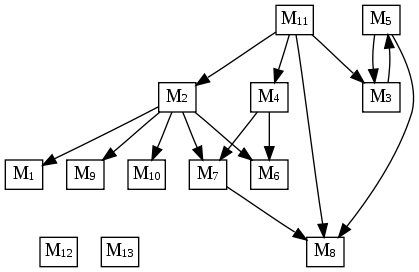
\includegraphics[width=1\columnwidth]{arquitetura-villonanny}
\par\end{centering}

\caption{\selectlanguage{brazil}%
Arquitetura modular extraída do sistema VilloNanny.\selectlanguage{portuges}
}
\label{fig:arquitetura-villonanny}


\end{figure}



\subsection{Escolha de Parâmetros e Síntese de Redes}

Queremos gerar redes com medidas próximas às medidas da rede de referência,
e isso depende de uma escolha adequada dos parâmetros dos modelos.


No modelo LFR os valores dos parâmetros $|V|$, $\langle k\rangle$,
$k_{max}$, $\gamma$, $\beta$, $t_{min}$ e $t_{max}$ coincidem
com os valores das métricas correspondentes extraídas da rede de referência.
O parâmetro de mistura, $\mu$, foi calculado segundo a equação $\mu=|E_{ext}|~/~|E|$,
onde $|E_{ext}|$ e $|E|$ são, respectivamente, o número de arestas
externas e o número total de arestas da rede de referência. A seguir
são listados os valores escolhidos para os parâmetros do modelo LFR:
$|V|=1658;\;\langle k\rangle=6,92;\; k_{max}=80;\;\gamma=2,68;\;\beta=1,00\;\mu=0,54;\; t_{min}=6;\; t_{max}=446$.

Para o modelo BCR+ utilizamos a arquitetura modular da Figura \ref{fig:arquitetura-villonanny},
extraída da rede de referência. Como estamos ignorando o sentido das
arestas, consideramos $p=q$ e $\delta_{in}=\delta_{out}$. Feita
essa restrição, ajustamos os parâmetros por tentativa e erro e chegamos
aos seguintes valores: $|V|=1658;\; p=q=0,1;\; r=0,8;\;\mu=0,09;\;\delta_{in}=\delta_{out}=3$.

Escolhidos os parâmetros, geramos nove redes a partir de cada modelo
e extraímos métricas. A Tabela \ref{tab:discrepancias} mostra a discrepância
entre as medidas da rede de referência e as médias das medidas das
redes sintetizadas por cada modelo. Na maioria dos casos a discrepância
pode ser creditada ao tamanho das redes, relativamente pequeno ---
os modelos garantem que as medidas se aproximam da medida esperada
quando o tamanho da rede tende a infinito. Em dois casos, no entanto,
a discrepância foi maior do que 5\%, o que sugere que a escolha dos
parâmetros pode ser aprimorada.

%
\begin{table*}
\caption{\selectlanguage{brazil}%
Discrepâncias relativas entre as medidas das redes sintéticas (média)
e as medidas da rede de referência.\selectlanguage{portuges}
}


\begin{centering}
\begin{tabular}{l|ccccc}
\hline 
 & \textbf{$|E|$ } & \textbf{$|E_{ext}|$ } & \textbf{$|M|$ } & \textbf{$\gamma$ } & \textbf{$\beta$ }\tabularnewline
\hline
\hline 
LFR\textbf{ } & 0,44\%  & 0,06\%  & 27,35\%  & 4,10\%  & 4,44\% \tabularnewline
BCR+\textbf{ } & 2,45\%  & 2,17\%  & 0,00\%  & 19,69\%  & 1,67\% \tabularnewline
\hline
\end{tabular}\label{tab:discrepancias}
\par\end{centering}
\end{table*}



\subsection{Cálculo da Distância Entre as Redes}

Após a extração das redes reais e da produção de redes sintéticas,
calculamos as distâncias entre a rede de referência e todas as demais
redes. Os resultados, agregados por modelo, podem ser vistos na Tabela
\ref{tab:distancias}. Os dados mostram que o modelo BCR+ foi o que
mais se aproximou da rede de referência; uma das redes geradas ficou
mais próxima à rede de referência do que a rede do sistema JFreeChart.
O modelo LFR produziu redes próximas entre si, como revela o pequeno
desvio-padrão, porém mais distantes da rede de referência.

%
\begin{table}
\caption{\selectlanguage{brazil}%
Distâncias das redes sintéticas e da rede do sistema JFreeChart em
relação à rede de referência.\selectlanguage{portuges}
}


\begin{centering}
\begin{tabular}{l|cc}
\hline 
Modelo/  & Distância & Distância \tabularnewline
Sistema & Média & Mínima\tabularnewline
\hline
\hline 
LFR  & $3,28\pm0,01$  & $3,26$ \tabularnewline
BCR+  & $2,60\pm0,28$  & $2,16$ \tabularnewline
JFreeChart  & $2,44\pm0,00$  & $2,44$ \tabularnewline
\hline
\end{tabular}\label{tab:distancias}
\par\end{centering}
\end{table}



\subsection{Ameaças à Validade}

Os resultados são bastante animadores, mas precisam ser analisados
à luz de algumas limitações do experimento:

\begin{itemize}
\item apenas dois sistemas reais foram estudados, e por isso, os resultados
não podem ser generalizados;
\item a métrica de distância ignora a organização das redes em módulos;
assim, nada se pode afirmar sobre o realismo das associações entre
vértices e módulos;
\item muitos algoritmos de modularização de \emph{software} operam sobre
redes orientadas e ponderadas, que contêm mais informação do que as
redes não-orientadas que analisamos.
\end{itemize}

\section{Discussão\label{sec:discussao}}

Este artigo apresentou uma nova abordagem, baseada na geração de sistemas
de \emph{software} sintéticos, de avaliação de algoritmos de modularização
de \emph{software}. Dois modelos de sistemas sintéticos foram apresentados
e avaliados através de um experimento. O experimento mostrou que o
modelo BCR+, proposto neste artigo, é capaz de sintetizar sistemas
semelhantes a sistemas reais. Esse resultado aumenta nossa confiança
na abordagem. 

Não defendemos que os sistemas sintéticos devem substituir completamente
os sistemas reais no teste de algoritmos de modularização de \emph{software},
mas acreditamos que eles podem proporcionar novas percepções sobre
os algoritmos. Além de fornecerem um grande volume de dados para teste,
eles permitem que se estude como a acurácia dos algoritmos é afetada
por variações nos parâmetros dos modelos. Lancichinetti, Fortunato
e Radicchi, por exemplo, estudaram dois algoritmos de modularização
de redes e mostraram que eles apresentam resultados piores quando
aplicados a redes com baixo grau médio \citep{Lancichinetti2008}.

Acreditamos que modelos de \emph{software} pode beneficiar pesquisas
em outras áreas de engenharia reversa, tais como análise de impacto
e localização de funcionalidades. A avaliação de ferramentas de engenharia
reversa em geral depende da disponibilidade de informações sobre sistemas
que não são representadas explicitamente em seu código-fonte. No caso
de localização de funcionalidades, por exemplo, essa informação é
o mapeamento entre as estruturas da implementação de um sistema e
as suas funcionalidades. Se esse mapeamento for incorporado em um
dos modelos aqui apresentados, então será possível testar as ferramentas
de localização de funcionalidades com um grande volume de dados.

Dois modelos de redes propostos recentemente, LR e CGW, deverão ser
avaliados em um trabalho futuro. O modelo LR é uma extensão do modelo
LFR para redes orientadas e ponderadas \citep{Lancichinetti2009}.
Já o modelo CGW produz redes orientadas através de um processo incremental
que inclui remoção e religamento de arestas \citep{Chen2008}. 

O próximo passo da pesquisa é realizar experimentos com a aplicação
de algoritmos de modularização de \emph{software} a redes sintéticas.
Os resultados desse experimento poderão ser comparados com os resultados
de experimentos já realizados com sistemas reais.

\bibliographystyle{abbrv}
\bibliography{complex-networks,rodrigo-mestrado}





\end{document}
